\chapter{Implementierung}
\label{implementation}
Das Programm ist komplett in C++ geschrieben und erfüllt die Anforderungen der Aufgabenstellung. Mit dem Programm ist es möglich, die gegebenen Beispieldaten einzulesen und mit dem Dempster Algorithmus eine Emotion (dessen Plausibilität am höchsten ist) für jeden Takt zu bestimmen. 
Die Ergebnisausgabe wird in der Konsole angezeigt und anschließend wird automatisch eine .CSV Datei geschrieben, in der die Ergebnisausgabe tabellarisiert ist. 


Das Programm kann in vier Teile eingeteilt werden.

\begin{enumerate}
  \item Einlesen der Beispieldaten aus den CSV-Dateien,
  \item Erstellen der Evidenzen für Sprechgeschwindigkeit (\(m_1\)), Tonlage (\(m_2\)) und Schallstärke (\(m_3\)),
  \item Verarbeiten der Evidenzen (Bilden von \(m_{123}\) und Berechnung der Plausibilität) und
  \item Ergebnisausgabe (Schreiben in eine CSV-Datei).
\end{enumerate}

Dabei ist jegliches, relevanter Codesegment im Quellcode kommentiert. 

Dieses Kapitel befasst sich vorerst mit der Dateistruktur der Implementation. Daraufhin wird jede Datei einzeln betrachtet und anschließend noch die Datenstruktur der Evidenzen erläutert.  

\section{Dateistruktur}
Das Programm ist in drei Dateien aufgeteilt:

\begin{description}
  \item [Main.cpp] Diese Datei verlinkt die anderen beiden Dateien und dient als Startpunkt. 
  \item [settings.h] In dieser Datei finden sich jegliche voreingestellten Makros, globale Initialisierungen, Konstanten und Variablen für das Programm. Die Headerdatei wird in Main.cpp und dempster.h eingebunden.
  \item [dempster.h] Diese Datei beinhaltet die Dempsterfunktion, welche von der Main.cpp aufgerufen wird.
  \end{description}

 Der verbleibende Teil dieser Dokumentation fokussiert sich nacheinander auf jede, genannte einzelne Datei und bespricht die implementierten Funktionen.

\section{settings.h}
Die Voreinstellungen des Programmes können in drei Teile eingeteilt werden.

Der erste Teil beinhaltet die Pfade zu den Beispiel-Eingabedaten (\verb|E_004.csv| und \verb|E_004b.csv|) und den jeweiligen Ausgabedaten. Zusätzlich kann noch ein Index angegeben werden, an welchem die Daten in den Dateien starten (um beispielsweise den Header zu überspringen).

Im zweiten Teil können die Konfidenzwerte (die Gewichtung der Evidenzen) festgelegt werden, welche in Kapitel \ref{konfidenzfestlegung} besprochen wurden. 

Im dritten Teil sind jegliche Werte der Ausprägungen festgelegt. Beispielsweise kann hier festgelegt werden, welcher Wert für den unteren Teil der Sprechgeschwindigkeit ausschlaggebend ist (Kapitel \ref{sprechgeschwindigkeit_auspr}) und wie die Ausprägungen der Merkmale in den vorgegeben Daten gespeichert sind.

\section{dempster.h}
In dieser Datei sind alle unmittelbar mit der Evidenzberechnung zusammenhängenden Funktionen zu finden. Die \textit{Dempster}-Funktion erwartet alle Evidenzen (\(m_1\), \(m_2\) und \(m_3\)) mit Gewichtung und akkumuliert sie zur finalen Evidenz \(m_{123}\). Des Weiteren beinhaltet sie eine Funktion zur Berechnung der \textit{Plausibilitäten}.

Zur Berechnung der Evidenzen wird das folgende Strukt benutzt:

\begin{lstlisting}[caption=Strukt zur Evidenzberechnung, label=structcode]
struct Evidence {
	Evidence() {}
	set<string> emotions;
	double value = 0.0;
};
\end{lstlisting}


Entscheidend sind hier das Set und der double-Wert. \textit{Evidence.emotions} beinhaltet alle zu dieser Evidenz gehörenden Emotionen (beispielsweise \textit{Wut} und \textit{Freude}) und kann auch leer sein, und \textit{Evidence.value} speichert die dazugehörige Konfidenz. Das entsprechende Omega wird mit dem gleichen Strukt gespeichert; \textit{emotions} beinhaltet hierbei alle Emotionen und \textit{value} ist \(1 - (Konfidenz der Evidenz)\). Die Evidenz und das dazugehörige Omega werden in einem Vektor mit mindestens zwei Komponenten gespeichert (oder mehr, falls Resultat einer Akkumulation). Dies ist in Diagramm \ref{diagramm_evidenzen} erkennbar.

\begin{figure}
\centering
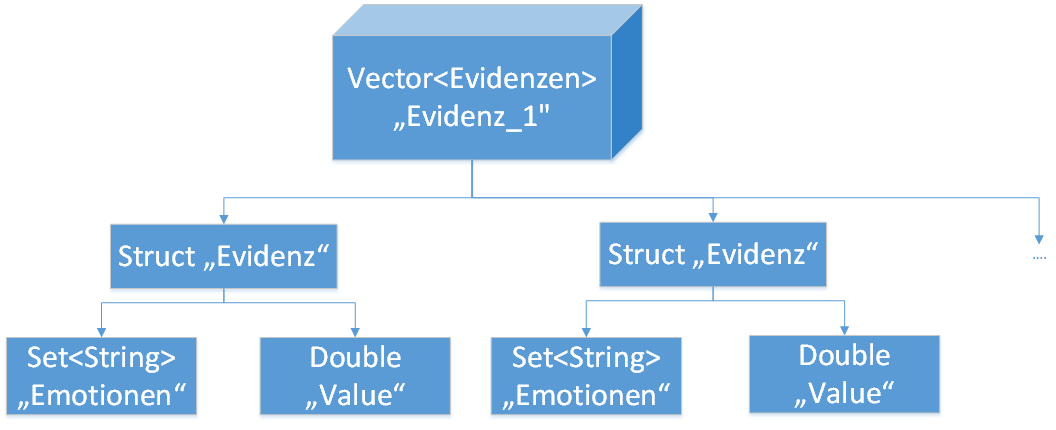
\includegraphics[width=\textwidth]{images/Evidenzen_diagramm.pdf}
\caption{Struktur der Evidenzen}
\label{diagramm_evidenzen}
\end{figure}

In der \textit{Dempster}-Funktion wird zuerst aus \(m_1\) und \(m_2\) die Evidenz \(m_{12}\) durch Vereinigung der Sets und Multiplikation der Konfidenzen gebildet, und es entstehen vier mögliche Kombinationen. Anschließend wird die Kombination aus Evidenz von \(m_1\) und \(m_2\) auf einen Konflikt untersucht; sollte ein Konflikt auftreten, wird \(k\) gebildet, die entsprechende leere Menge aus \(m_{12}\) entfernt und die übrigen Konfidenzen mit \(\frac{1}{1-k}\) korrigiert. Durch Akkumulation von \(m_{12}\) und \(m_3\) entsteht auf gleichem Wege \(m_{123}\), und die resultierenden Mengen werden auf Konflikte untersucht, diese gegebenenfalls gelöscht und der Rest korrigiert. Die Funktion wird einmal pro Takt aufgerufen.
 
Die Plausibilitätsberechnung geschieht in der Funktion \verb|plausibility()|. Als Eingabeparameter wird hier die Evidenz \(m_{123}\) erwartet. Durch Iterieren über alle Teilevidenzen werden für jede Emotion die Teilwerte aufsummiert und in einen neuen Vektor gespeichert. Anschließend wird die größte Plausibilität gesucht und zusätzlich abgespeichert.
 
\section{Main.cpp}
Die Main.cpp Datei beinhaltet die \textit{Main-Funktion}, welche bei Programmstart aufgerufen wird.
Zusätzlich zu der Main-Funktion sind hier weitere Funktionen zu finden. Der folgende Ausschnitt zeigt jegliche Funktionssignaturen der Main.cpp befindet sich im Abschnitt \textit{Predefined Functions} dieser Datei: 

\begin{lstlisting}[caption=Predefined classes/functions aus der Main.cpp, label=Bsp.1]
double toDouble(string s);
void printFile(string filename);
vector<string> readFileInVector(string filename);
void writeResultsToFile(string filename, 
	vector<vector<Evidence>> evidences, 
	vector<map<string, double>> plausibilities);
void printAverageSpeed(vector<string> data);
set<string> getEmotionOfSpeed(double);
set<string> getEmotionOfPitch(string);
set<string> getEmotionOfIntensity(string);
void calculatePlausibilities(string input, string output);
\end{lstlisting}
Die Funktionen \verb|printFile()|, \verb|readFileInVector| und \verb|writeResultsToFile()| sind  für Dateieingabe und -ausgabe zuständig. Mit \verb|printAverageSpeed()| wurde die durchschnittliche Sprechgeschwindigkeit bestimmt. \verb|getEmotionOfSpeed()|, \verb|getEmotionOfPitch()| und \verb|getEmotionOfIntensity()| liefern die Emotionen anhand der Eingabewerte entsprechend der Tabelle \ref{tab:konkretisierteEmotionen}. In der Funktion \verb|calculatePlausibilities()| befindet sich das Hauptprogramm bestehend aus Aufruf der Einlesefunktionen, einer Schleife, die für jeden Takt die \textit{Dempster}-Funktion aufruft und dem Aufruf der Ausgabefunktion.

%Die Funktion \textit{calculate\_plausibilities} ruft vorerst die Funktion \textit{readFileInVector} um die Daten zu lesen, die Dempster-Funktion in der dempster.h Datei um die Daten auszuwerten und daraufhin die Funktion \textit{writeResultsToFile} damit das Ergebnis in eine Datei geschrieben wird. Die Funktionen in Zeile 8,9 und 10, welche mit \textit{getEmotion} beginnen, sind dazu dar, um aus den Beispieldaten die Emotionen zu extrahieren. Die Funktion \textit{printAverageSpeed} analysiert die Werte der Sprechgeschwindigkeit und gibt den Durchschnittswert und weitere nützliche Informationen in der Konsole aus.

%\section{Datenstruktur der Evidenzen}
%Da die Datenstruktur der Evidenzen nicht banal ist, wird diese an diesem Punkt der Dokumentation, näher beschrieben. Das Diagramm \ref{diagramm_evidenzen} zeigt die Struktur der Evidenzen dar. In dem Diagramm ist zu sehen, dass eine Evidenz drei verschiedenen Datentypen besteht. In der untersten Ebene befindet sich ein \textit{Set} aus Emotionen, welche als Strings in der Menge gespeichert sind. Zugehörig zu dieser Menge, ist ein Dezimalwert als \textit{Double} gespeichert. Diese beiden Datentypen werden über den Datentyp \textit{Struct} verbunden. Dabei beinhaltet eine Evidenz mindestens zwei Structs, kann jedoch mehr beinhalten. Mehrere Structs werden daraufhin über einen \textit{Vector} verbunden.

